A concern that has arisen with the estimation of mortality change in the United States among white and black groups is that reporting patterns for Hispanic identity may have changed over recent decades. The Hispanic population of the U.S. has higher in- and out-migration, making mortality estimates for this group more difficult to measure \citep{Markides2005}.  Hispanics also have considerably lower mortality rates than other groups \citep{Palloni2004,Markides2005}. If patterns of Hispanic reporting change over time, and especially if they change differentially across the Current Population Survey and the Vital Statistics databases, then estimates of mortality change for non-Hispanics could be biased.

In this section, we consider and rule out two alternative hypotheses for the measured rise in non-Hispanic white mortality. First, survey questions change subtly over time; for example, the Census permitted people to check multiple race boxes starting in 2000 \citep{Currie2018}. We show that there are no discontinuities in the combined population records for non-Hispanic white or black populations in our sample, suggesting multiple race reporting is not substantially biasing mortality estimates.

Second, populations' attitudes about their own racial/ethnic identity may change over time. The same person might be more likely to report herself as a given race/ethnicity in 2018 than in 1992. Because Hispanics have lower mortality rates, if white Hispanics are more likely to report Hispanic identity over time in surveys, this phenomenon could bias the non-Hispanic mortality trend upward. We conduct a bounding exercise that shows that even if an implausibly large number of whites changed their identity to Hispanic, there would still be large mortality gains among less educated non-Hispanic whites.

Finally, average misalignment between Hispanic identification on death records and in census counts would not bias mortality estimates unless the error rate changed between 1992 and 2018. Further, researchers have examined potential misreporting of Hispanic identity on death certificates, and have found that reporting of identity on death certificates is in fact reliable and consistent with census data, with error rates consistently falling below 10\%, which is too low to explain the patterns described in this paper \citep{Rosenberg1999,Arias2008,Arias2010,Ruiz2013}.

\vspace{6mm} \textbf{Changes in survey questions.} The option to check
more than one race box in the 2000 Census has the potential to change
the share of the population that reports as any given race
\citep{Currie2018}. The CPS question on race changed in 2003, while
the question in the ACS (which we use only to calculate the
institutionalized population) changed in 2008.  Figure \ref{fig:pops}
plots the total population in our dataset by age and race. There is
clearly no large discontinuous change in the population of any group
in either of these years, suggesting that the option to check multiple
races in these national surveys cannot explain the secular trend in
rising mortality among the least educated white non-Hispanics. Note
also that only 5\% of white 20-year-olds in the 2010 Census report
multiple races \citep{Currie2018}. This number drops to less than 2\%
among white 50-year-olds. This is thus unlikely to be a major concern.

\vspace{6mm}

\textbf{Differences between the Census/CPS and NCHS reporting.} A
separate concern is that Hispanic identity could be reported
differently on death certificates and in Census counts. Misreporting
of ethnic identity on death certificates on average would not affect
our findings on mortality \textit{changes} unless the frequency of
misreporting changes substantially during the sample
period. For instance, to create an upward bias in mortality change
among non-Hispanic whites, Hispanic identity could be reported
correctly on death certificates in 1992 but substantially underreported
in 2018. In that case, there must be only small changes in accuracy of
reporting in the CPS. 

To test the extent to which changes in reporting of Hispanic identity could influence mortality estimates among non-Hispanic white mortality, we simulated misreporting in the data, focusing on non-Hispanic white women aged 50--54 in the least educated 10\%. Specifically, we assumed that X\% of white Hispanics in 2016--18 would have reported themselves as non-Hispanic white in 1992--94. We therefore reassigned X\% of white Hispanic deaths to be counted as white non-Hispanic deaths in 2016--18, and then recalculated bounds on mortality change from 1992--94 to 2016--18.  Panels A and B of Figure \ref{fig:hisp_changes} plot the results of this exercise for non-Hispanic white women and men respectively. Even in the extreme case where 20\% of white non-Hispanic female deaths in 2016--18 would have been reported as Hispanic deaths in 1992--94, we would still detect an increase in mortality of [397, 590] deaths per 100,000 among the bottom 10\%, putting the lower bound on mortality increase at 65\%. This example shows that even an extreme amount of misreporting could not drive our findings for the least educated group; however, note that estimates suggest the true amount of this kind of misreporting is much smaller than this extreme case \citep{Rosenberg1999,Arias2008,Arias2010,Ruiz2013}.

\begin{figure}[H]
  \caption{Population Counts by Group}
  \label{fig:pops}
  \begin{center}
    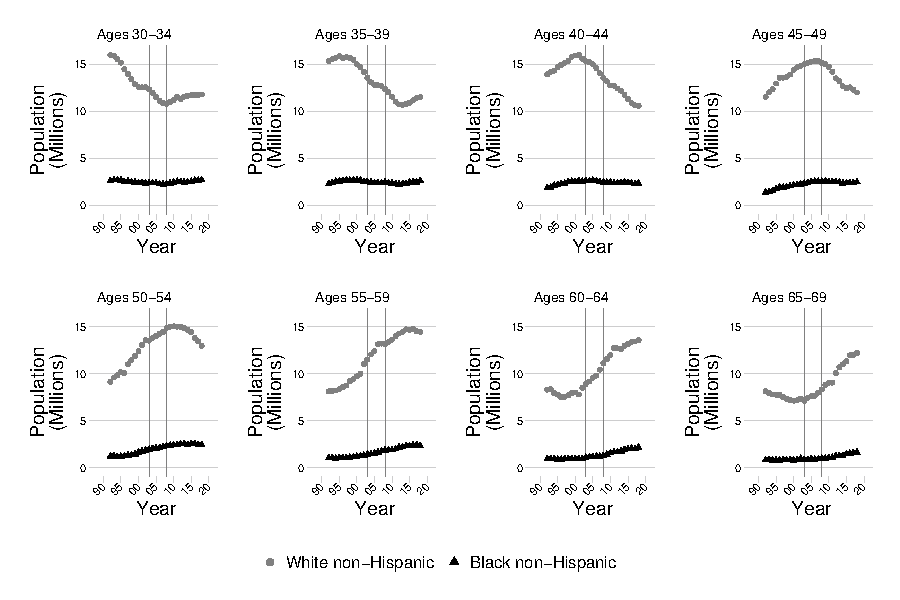
\includegraphics[scale=1.2]{\mortalitypath/total_pops} \\
  \end{center}
\end{figure}
\scriptsize{Note: the figure shows the population in each 5-year age bin of black and white non-Hispanics according to the CPS / ACS over the study sample period.}

\begin{figure}[H]
  \caption{Mortality Changes with Simulated Measurement Error}
  \label{fig:hisp_changes}
  \begin{center}
    \begin{tabular}{c}
      \small{Panel A: Non-Hispanic White Women Ages 50--54} \\ 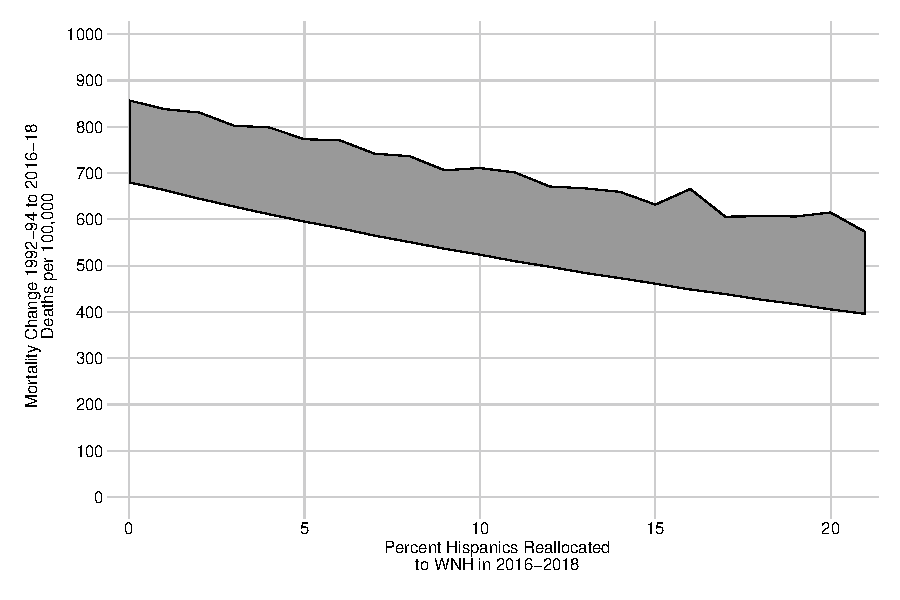
\includegraphics[scale=.75]{\mortalitypath/hisp_shift_2} \\
      \small{Panel B: Non-Hispanic White Men Ages 50--54} \\ 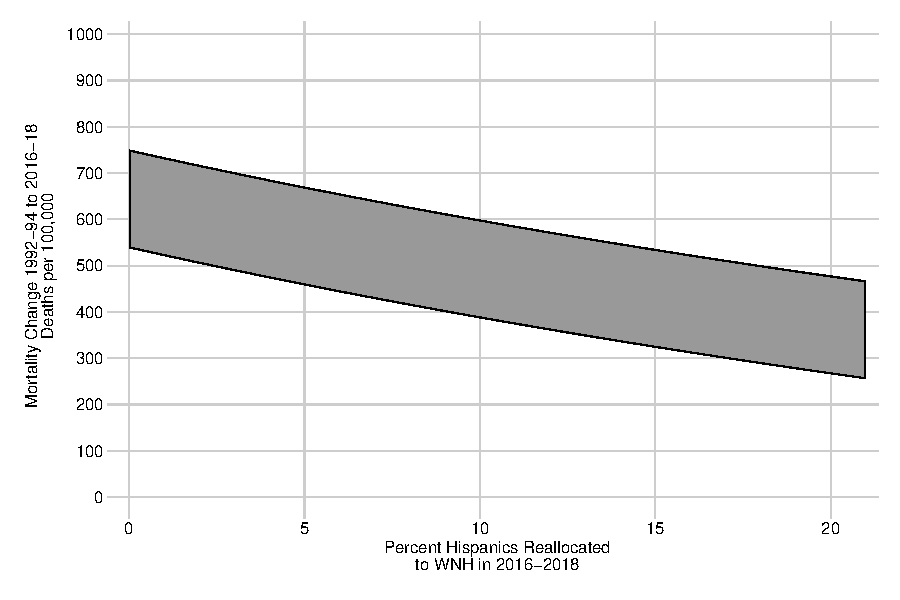
\includegraphics[scale=.75]{\mortalitypath/hisp_shift_1}
    \end{tabular}
  \end{center}
\end{figure}
\scriptsize{Note: The figure displays the sensitivity of mortality estimates to measurement error in ethnicity. The figure shows how primary mortality change estimates change if we recode white Hispanic deaths in 2016--18 to white non-Hispanic deaths, leaving reporting in 1992--94 and population totals unchanged. The X axis shows the percentage of Hispanic deaths recoded as non-Hispanic deaths under each scenario. The Y axis shows bounds on mortality change from 1992--1994 to 2016--2018 among non-Hispanic white men and women aged 50--54 in the least educated 10\%, under each different recoding. Bounds are otherwise calculated as in the body of the paper.}
